% !TEX root = Projektdokumentation.tex

% 	Die Einleitung soll allgemein verständlich sein, d.h. sie soll beispielsweise auch für Ihre Freunde und Verwandten verständlich sein. Sie stellt die Aufgabe in einen grösseren Zusammenhang und liefert eine genaue Beschreibung der Ausgangslage und Problemstellung. Allfällige Vorarbeiten oder ähnlich gelagerte Arbeiten sind diskutiert. Zum Schluss der Einleitung können Sie auch beschreiben, welche Abschnitte des Berichts sich an welche Leser wenden (z.B. Anwender des Produkts, Entwickler, Betreiber).


%Überprüfen von Wissen \\
Während dem Studium werden viele Inhalte vermittelt und anschliessend mit einer Schlussprüfung abgeholt. Wie merkt ein Student aber schon vor der Prüfung, ob sein Wissen sattelfest ist? Mobile Quiz bietet eine Lösung dafür. Der Dozent publiziert nach jeder Lektion Fragen zu den vermittelten Inhalten, welche die Studierenden online beantworten können. So erhalten Sie umgehend Feedback zu ihrem Wissensstand.
Die folgende Figur zeigt die wichtigsten Interaktionen der unterschiedlichen Benutzer mit dem Mobile Quiz:

\begin{figure}[H]
	\centering
	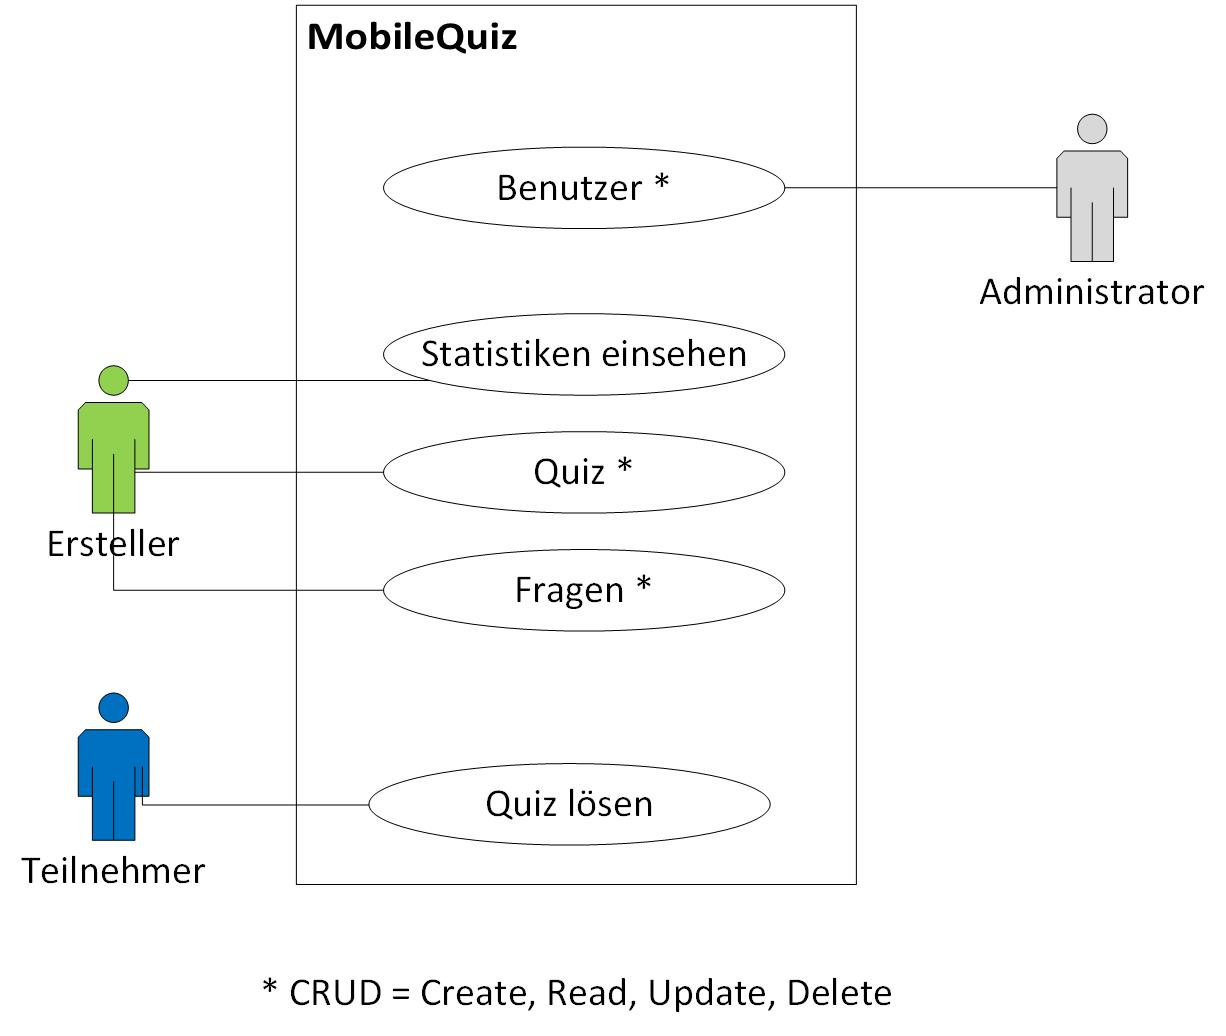
\includegraphics[width=0.75\textwidth]
	{Images/MobileQuiz_Uebersicht.PNG}
	\caption{Übersicht der wichtigsten Funktionen des Mobile Quiz}
\end{figure}

%Stand Mobile Quiz \\
Stand vor der Studienarbeit umfasst Mobile Quiz inzwischen einige Funktionen, um Quizzes zu erstellen. Verbesserungspotentiale liegen allerdings noch in den Bereichen der Bedienbarkeit, im Bereich von neuen Fragetypen sowie in der Auswertung von Quizzes. Durch letzteres wäre es dem Dozenten ersichtlich, welche Teile des Stoffs gut verstanden wurden und bei welchen noch Nachholbedarf herrscht. Somit könnte die Vorlesungszeit effizienter genutzt werden.
\todo{Andrea: Screenshots von alter Version um aufzuzeigen, was vorher schon bestanden hat und mit Link auf die alte Version verweisen.}
\\
%In dieser Arbeit wird XY umgesetzt.
\\
%Übersicht Kapitel \\

	\todo{Andrea}